\chapter{Related Work}\label{rltwrk}
In this chapter, some related work are illustrated in detail. Section \ref{dlimgseg} presents several deep learning networks for semantic and instance segmentation. Section \ref{frmgeo} introduces methods related to geometrical shapes extraction with and without machine learning frameworks. Section \ref{motivation} gives the summary of some of these models, points out their respective deficiencies with regard to our problem, and further discusses the feasibility of applying those models to our problem.

\section{Deep Learning for Image Segmentation}\label{dlimgseg}
This section mainly introduces some deep learning frameworks used in image segmentation. Subsection \ref{dlsemseg} and subsection \ref{dlistseg} focus on semantic and instance segmentation, respectively.

\subsection{Frameworks for Semantic Segmentation}\label{dlsemseg}
Traditional CNN-based semantic segmentation approach is usually done by classifying a pixel using the small neighboring patch centered on this pixel as input to the CNN. This method has several disadvantages such as the large storage, inefficient computing (patches of adjacent pixels are basically repeated) and the limitation of the sensing area (only local features can be extracted). However, the application of FCN (Fully Convolutional Networks) to semantic segmentation of images, which originates from this far-reaching paper \cite{fcn}, breaks with precedent. Figure \ref{fig:mdlfcn} shows the model architecture of FCN, and the core techniques used by FCN are also shown as follows.

\begin{figure}[!h]
	\centering
	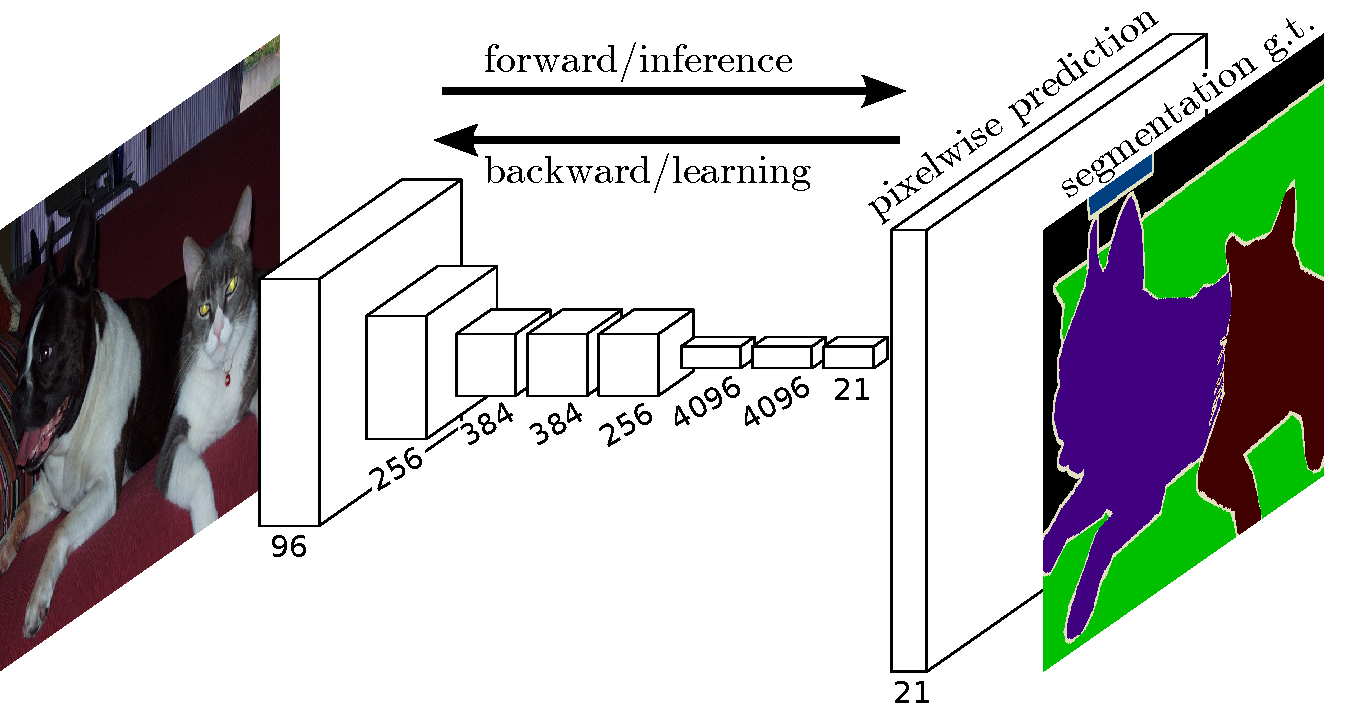
\includegraphics[width=\figfi\textwidth]{2-04.pdf}
    \caption[Model architecture of FCN]{Model architecture of FCN. Image copyright owned by \cite{fcn}.}
    \label{fig:mdlfcn}
\end{figure}

\paragraph{Convolutionalization}
The CNN used for image classification generally has fully connected layers at the end. It compresses the two-dimensional matrix into one-dimensional vector, thus losing the spatial information. In contrast, FCN discards those fully connected layers and replaces it with convolutional layers. This replacement is so-called convolution. The spatial output maps of these convolutionalized models make them a natural choice for dense problems like semantic segmentation. Figure \ref{fig:convfcn} shows the convolutionalization process.

\begin{figure}[!h]
	\centering
	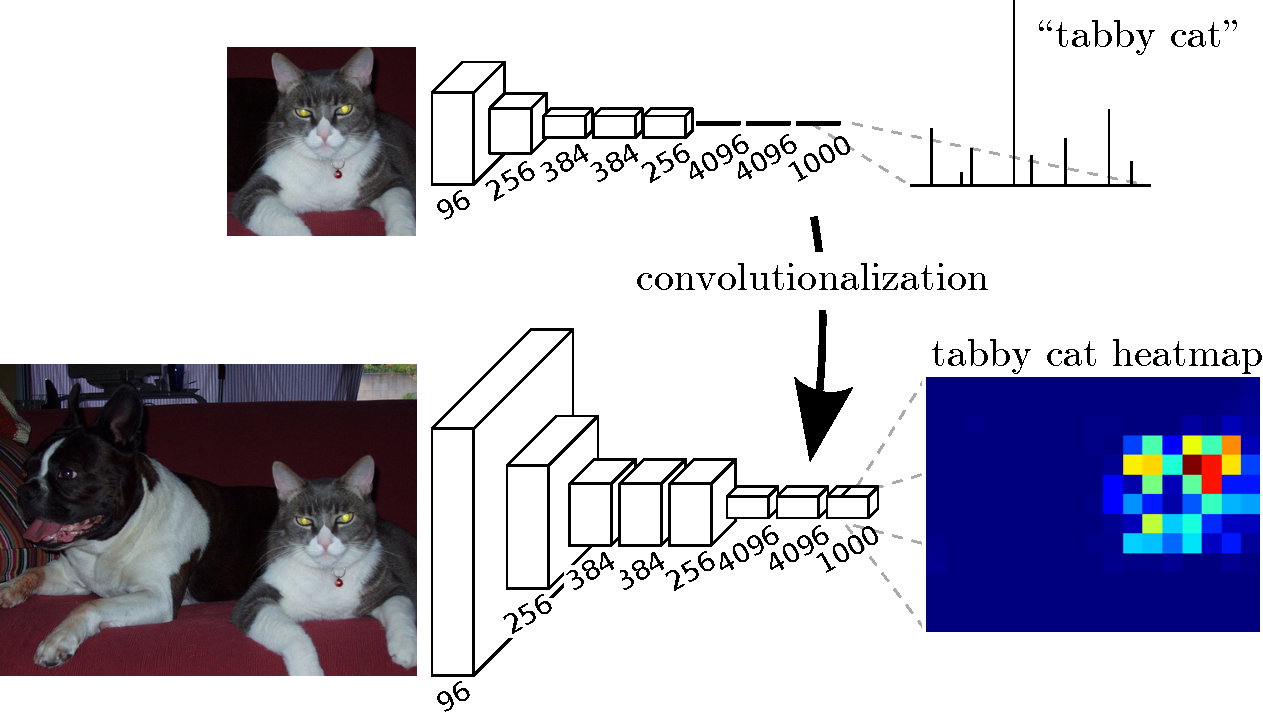
\includegraphics[width=\figfi\textwidth]{2-05.pdf}
    \caption[Convolutionalization in FCN]{Convolutionalization in FCN. Image copyright owned by \cite{fcn}.}
    \label{fig:convfcn}
\end{figure}

\paragraph{Upsampling}
In-network upsampling layers enable pixel-wise prediction and learning in nets with subsampled pooling. As we know, CNN uses several pooling layers to reduce the image size (usually the size is reduced by half for each pooling layer). However, in semantic segmentation, the mask with the same size as the original image is required. Hence, we need to perform upsampling, and the corresponding layer is so-called deconvolutional (transposed convolutional) layer. It shows that learning dense prediction through upsampling is more effective and efficient, especially when combined with the skip layer fusion \cite{fcn}.

\paragraph{Skip Connection}
Skip architecture combines semantic information from a deep, coarse layer with appearance information from a shallow, fine layer to produce accurate and detailed segmentations. Skip connection, which is shown in figure \ref{fig:skipfcn}, can take advantage of this feature spectrum and refine the spatial precision of the output.

\begin{figure}[!h]
	\centering
	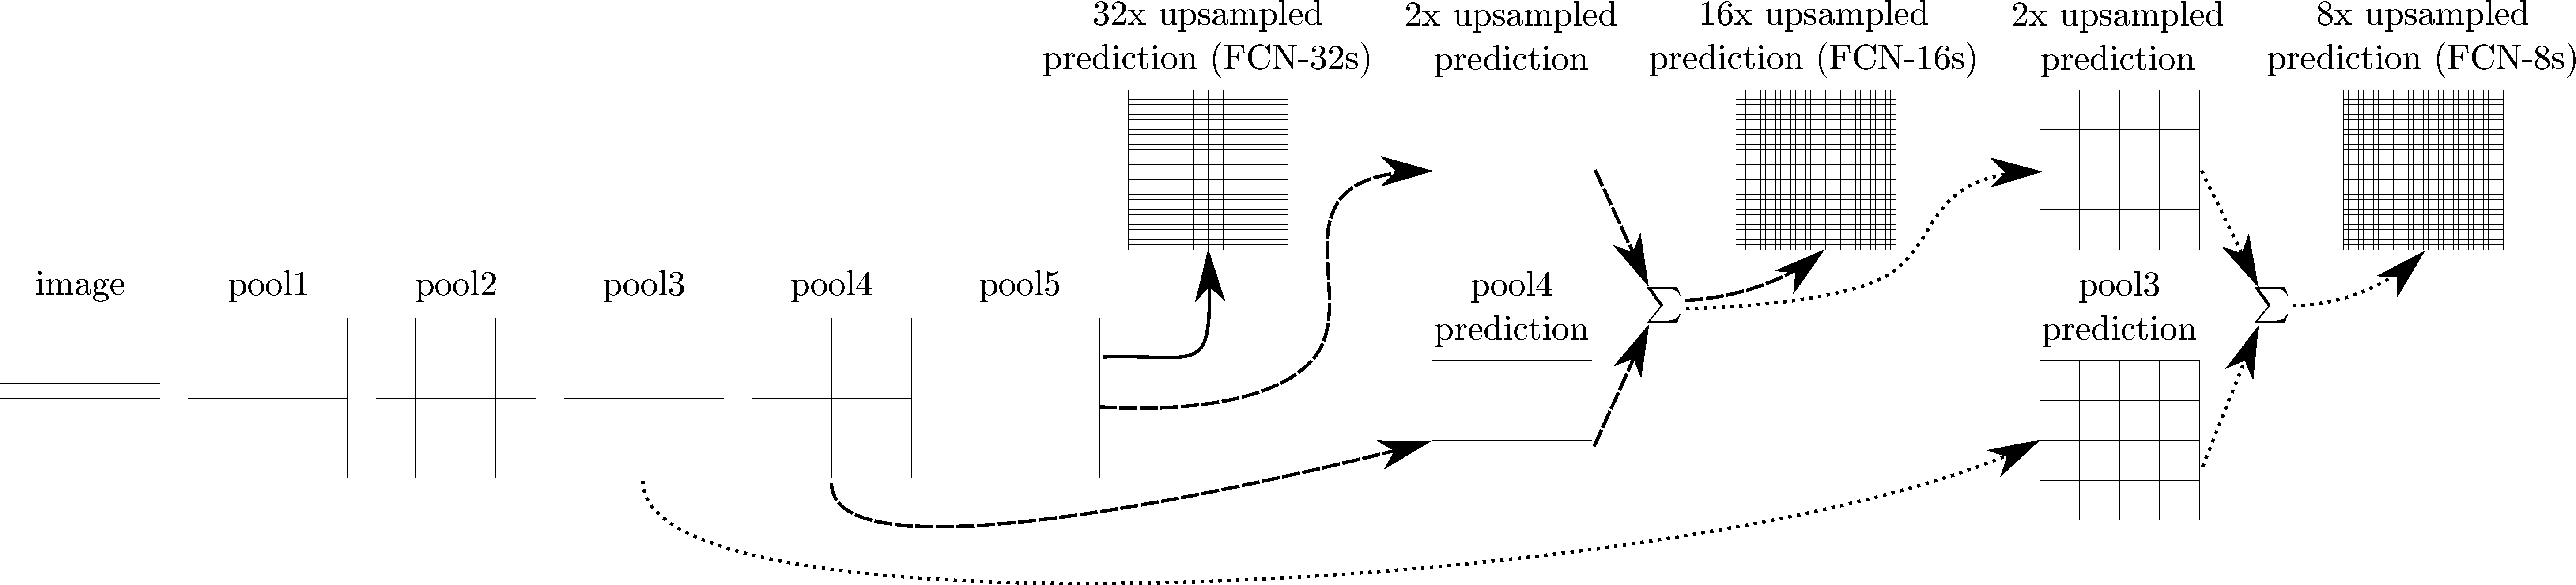
\includegraphics[width=\fig\textwidth]{2-06.pdf}
    \caption[Skip connection in FCN]{Skip connection in FCN. Image copyright owned by \cite{fcn}.}
    \label{fig:skipfcn}
\end{figure}

Compared with previous conventional method of semantic segmentation using CNN, FCN has two major advantages: (1) It can accept input image of arbitrary size, without stretching the image to a fixed size; (2) FCN is more efficient as it avoids the problem of duplicate in both storage and computation.

At the same time, the disadvantages of FCN are also obvious: (1) The results obtained are not precise enough, since upsampling makes the mask blurry and smooth, and it is not sensitive to the details in the image; (2) Pixel-wise classification does not fully consider the relationship between neighboring pixels, ignoring the spatial regularization used in general per-pixel segmentation methods, thus lacking spatial consistency.

In order to tackle the shortcomings mentioned above, many expansions of FCN are proposed such as DeepLab \cite{deeplab}, U-Net \cite{unet} and SegNet \cite{segnet}. Due to space limitations, in this thesis, we will not elaborate on all of these models. Please refer to the original paper for more details.

\begin{figure}[!h]
	\centering
	\subbottom[\label{fig:mspascal1}]{
		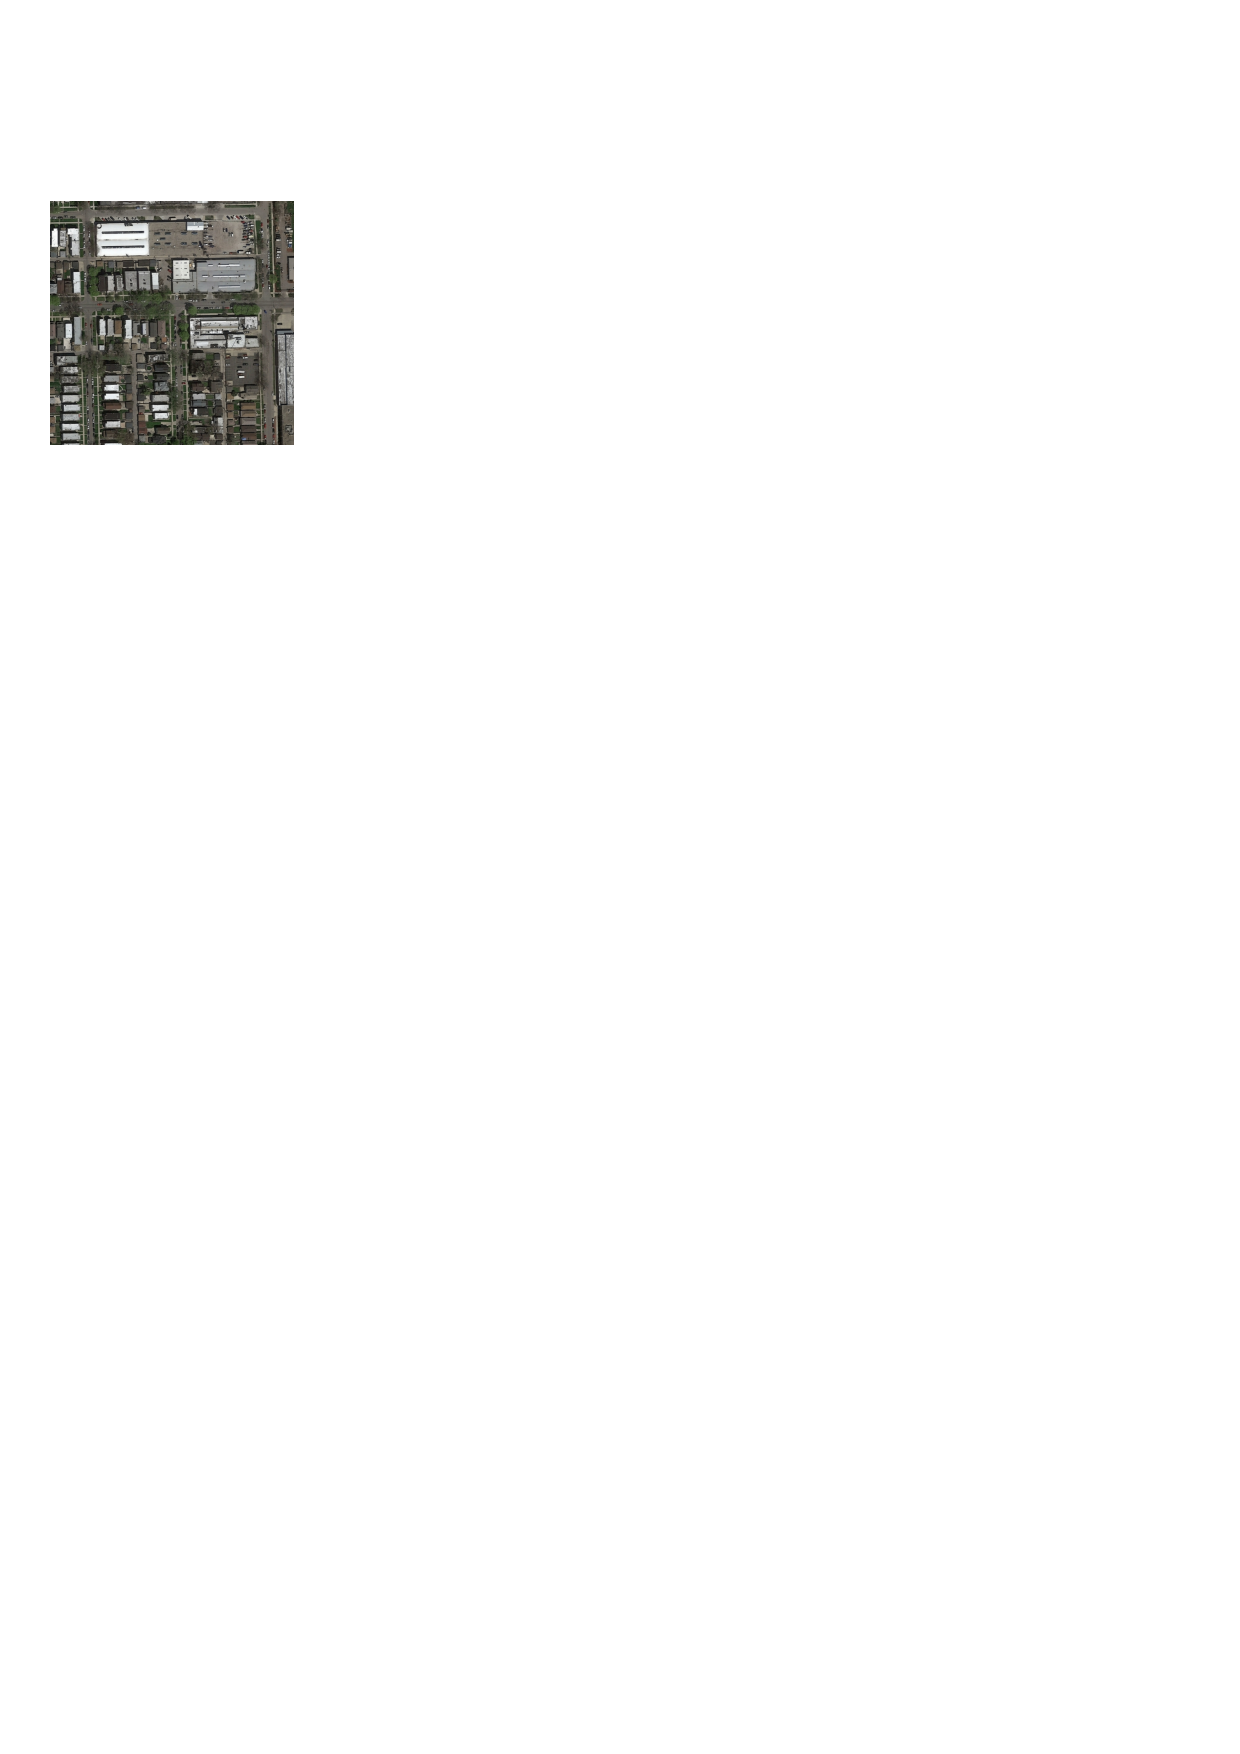
\includegraphics[width=\figfigfigfig\textwidth]{2-00-0.pdf}
	}
	\subbottom[\label{fig:mspascal2}]{
		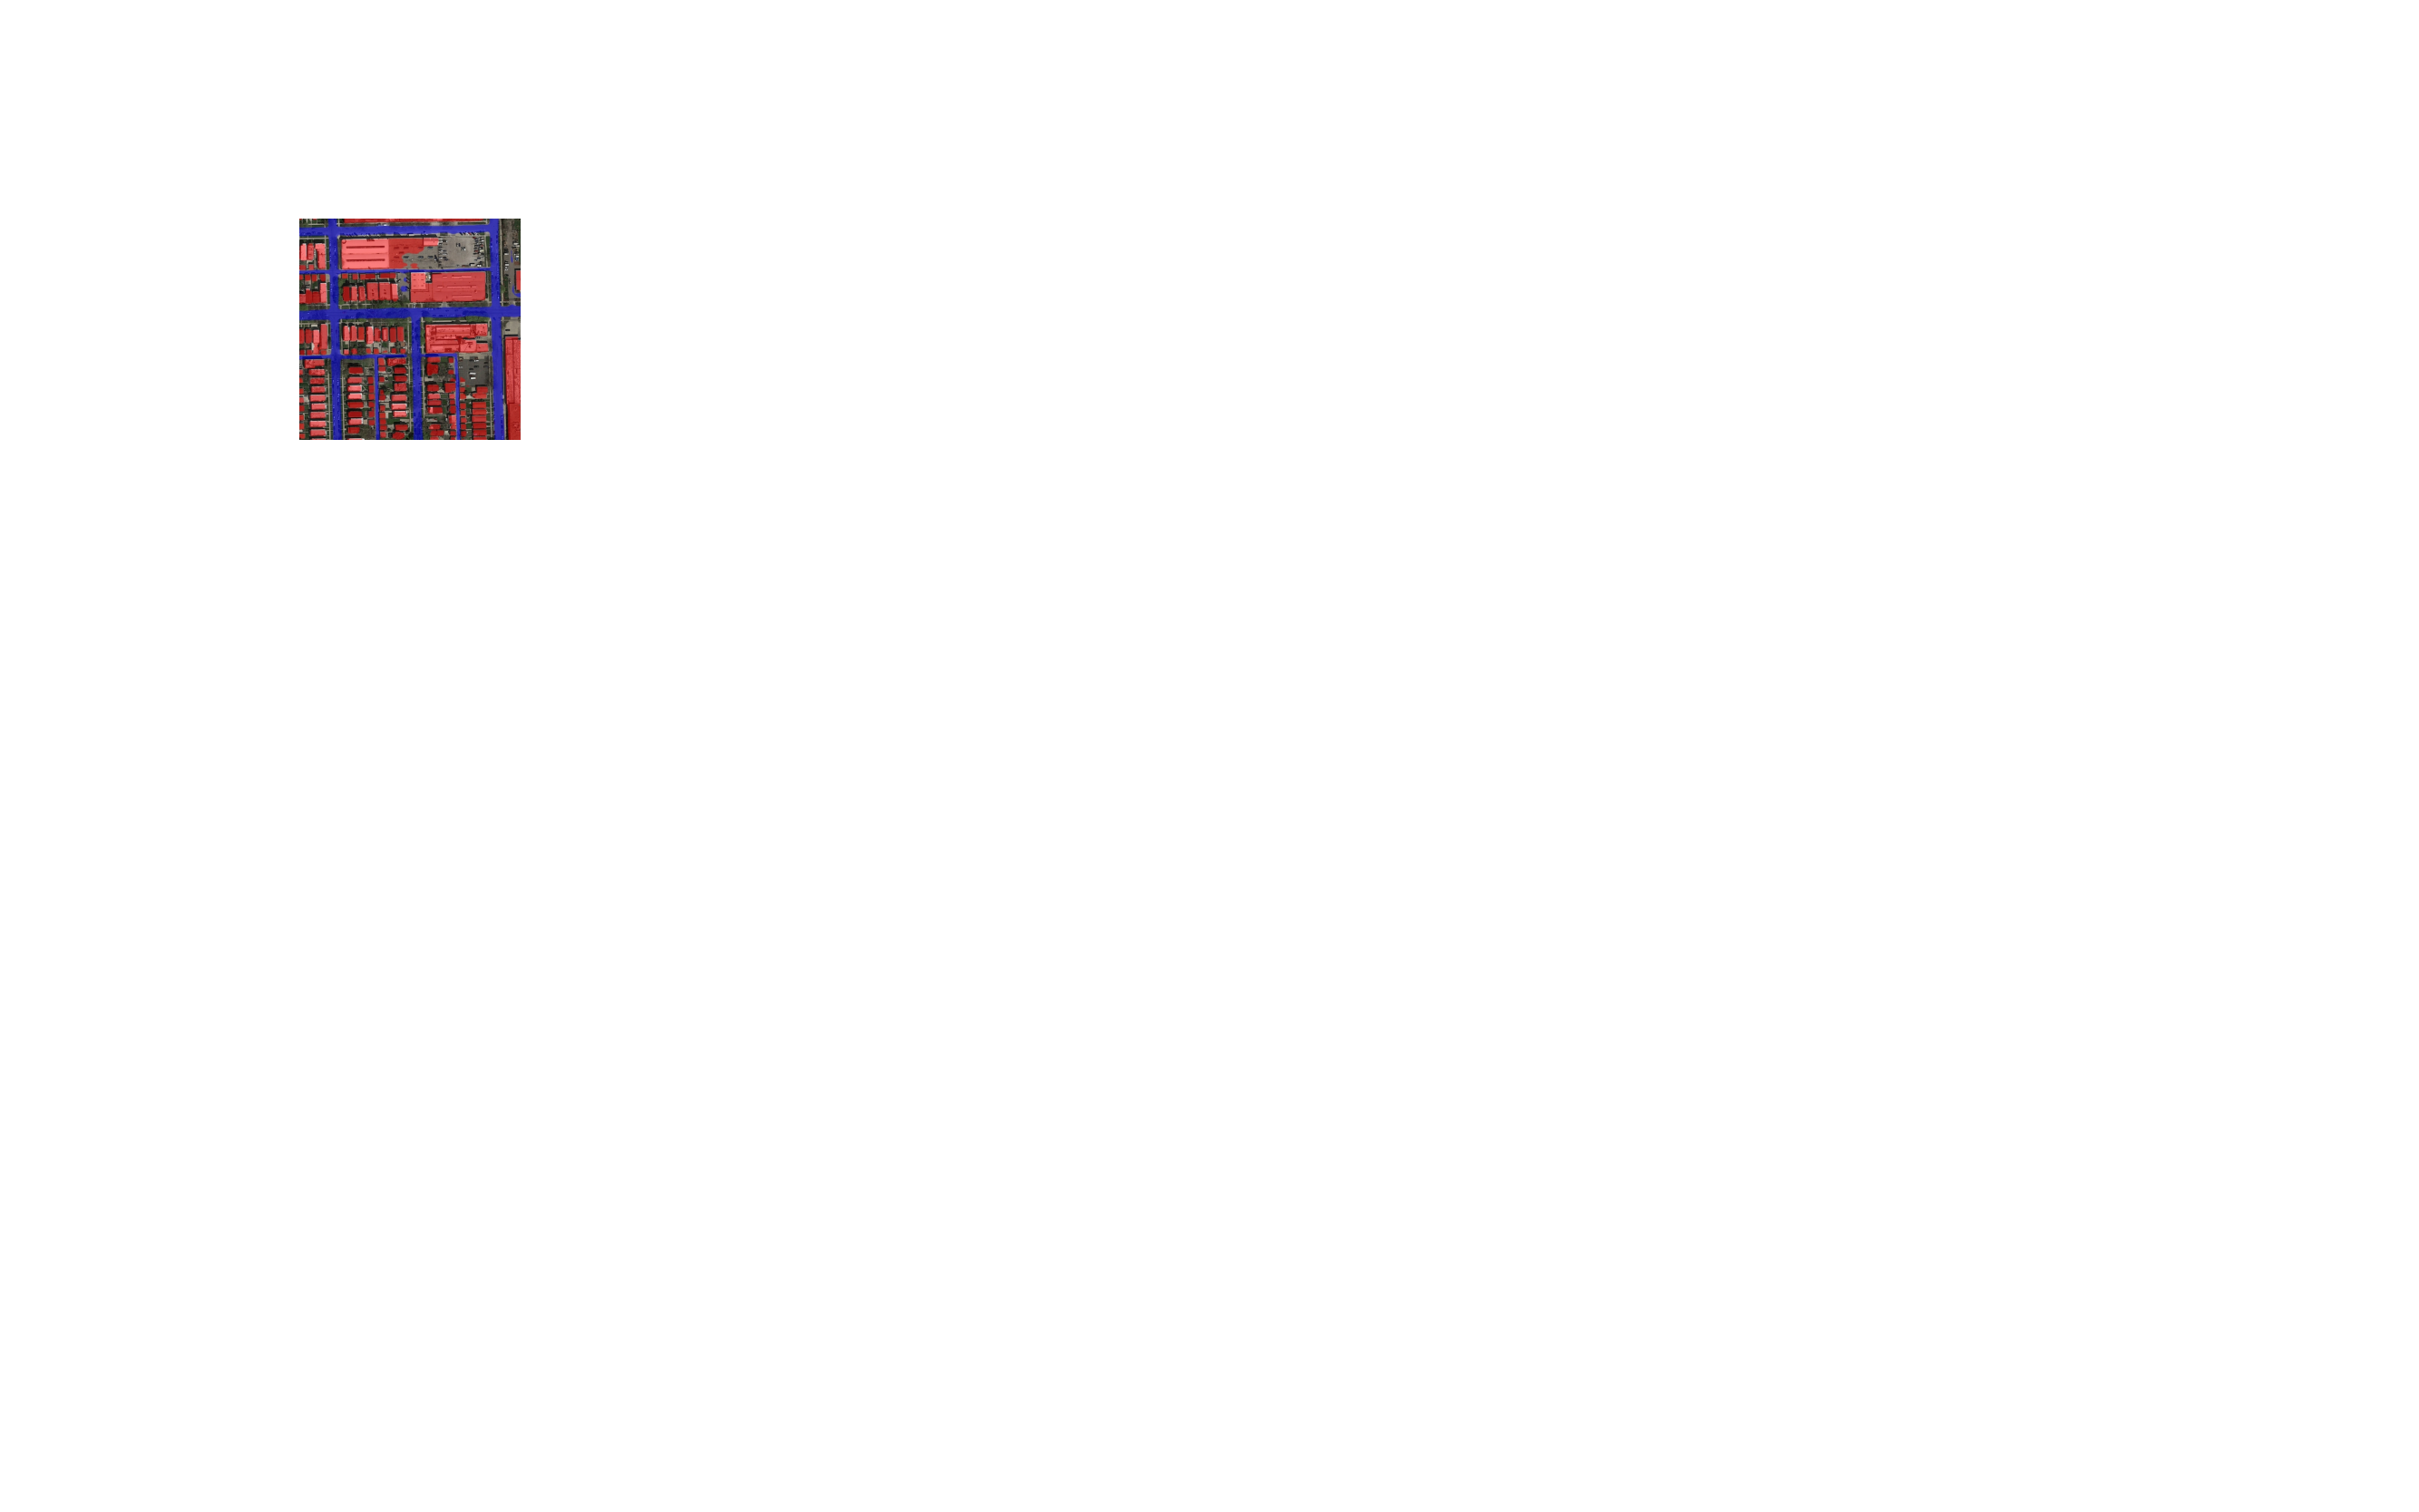
\includegraphics[width=\figfigfigfig\textwidth]{2-00-1.pdf}
	}
	\subbottom[\label{fig:mspascal3}]{
		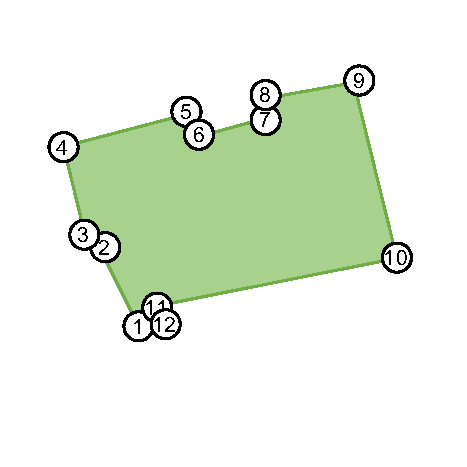
\includegraphics[width=\figfigfigfig\textwidth]{2-00-2.pdf}
	}
	\subbottom[\label{fig:mspascal4}]{
		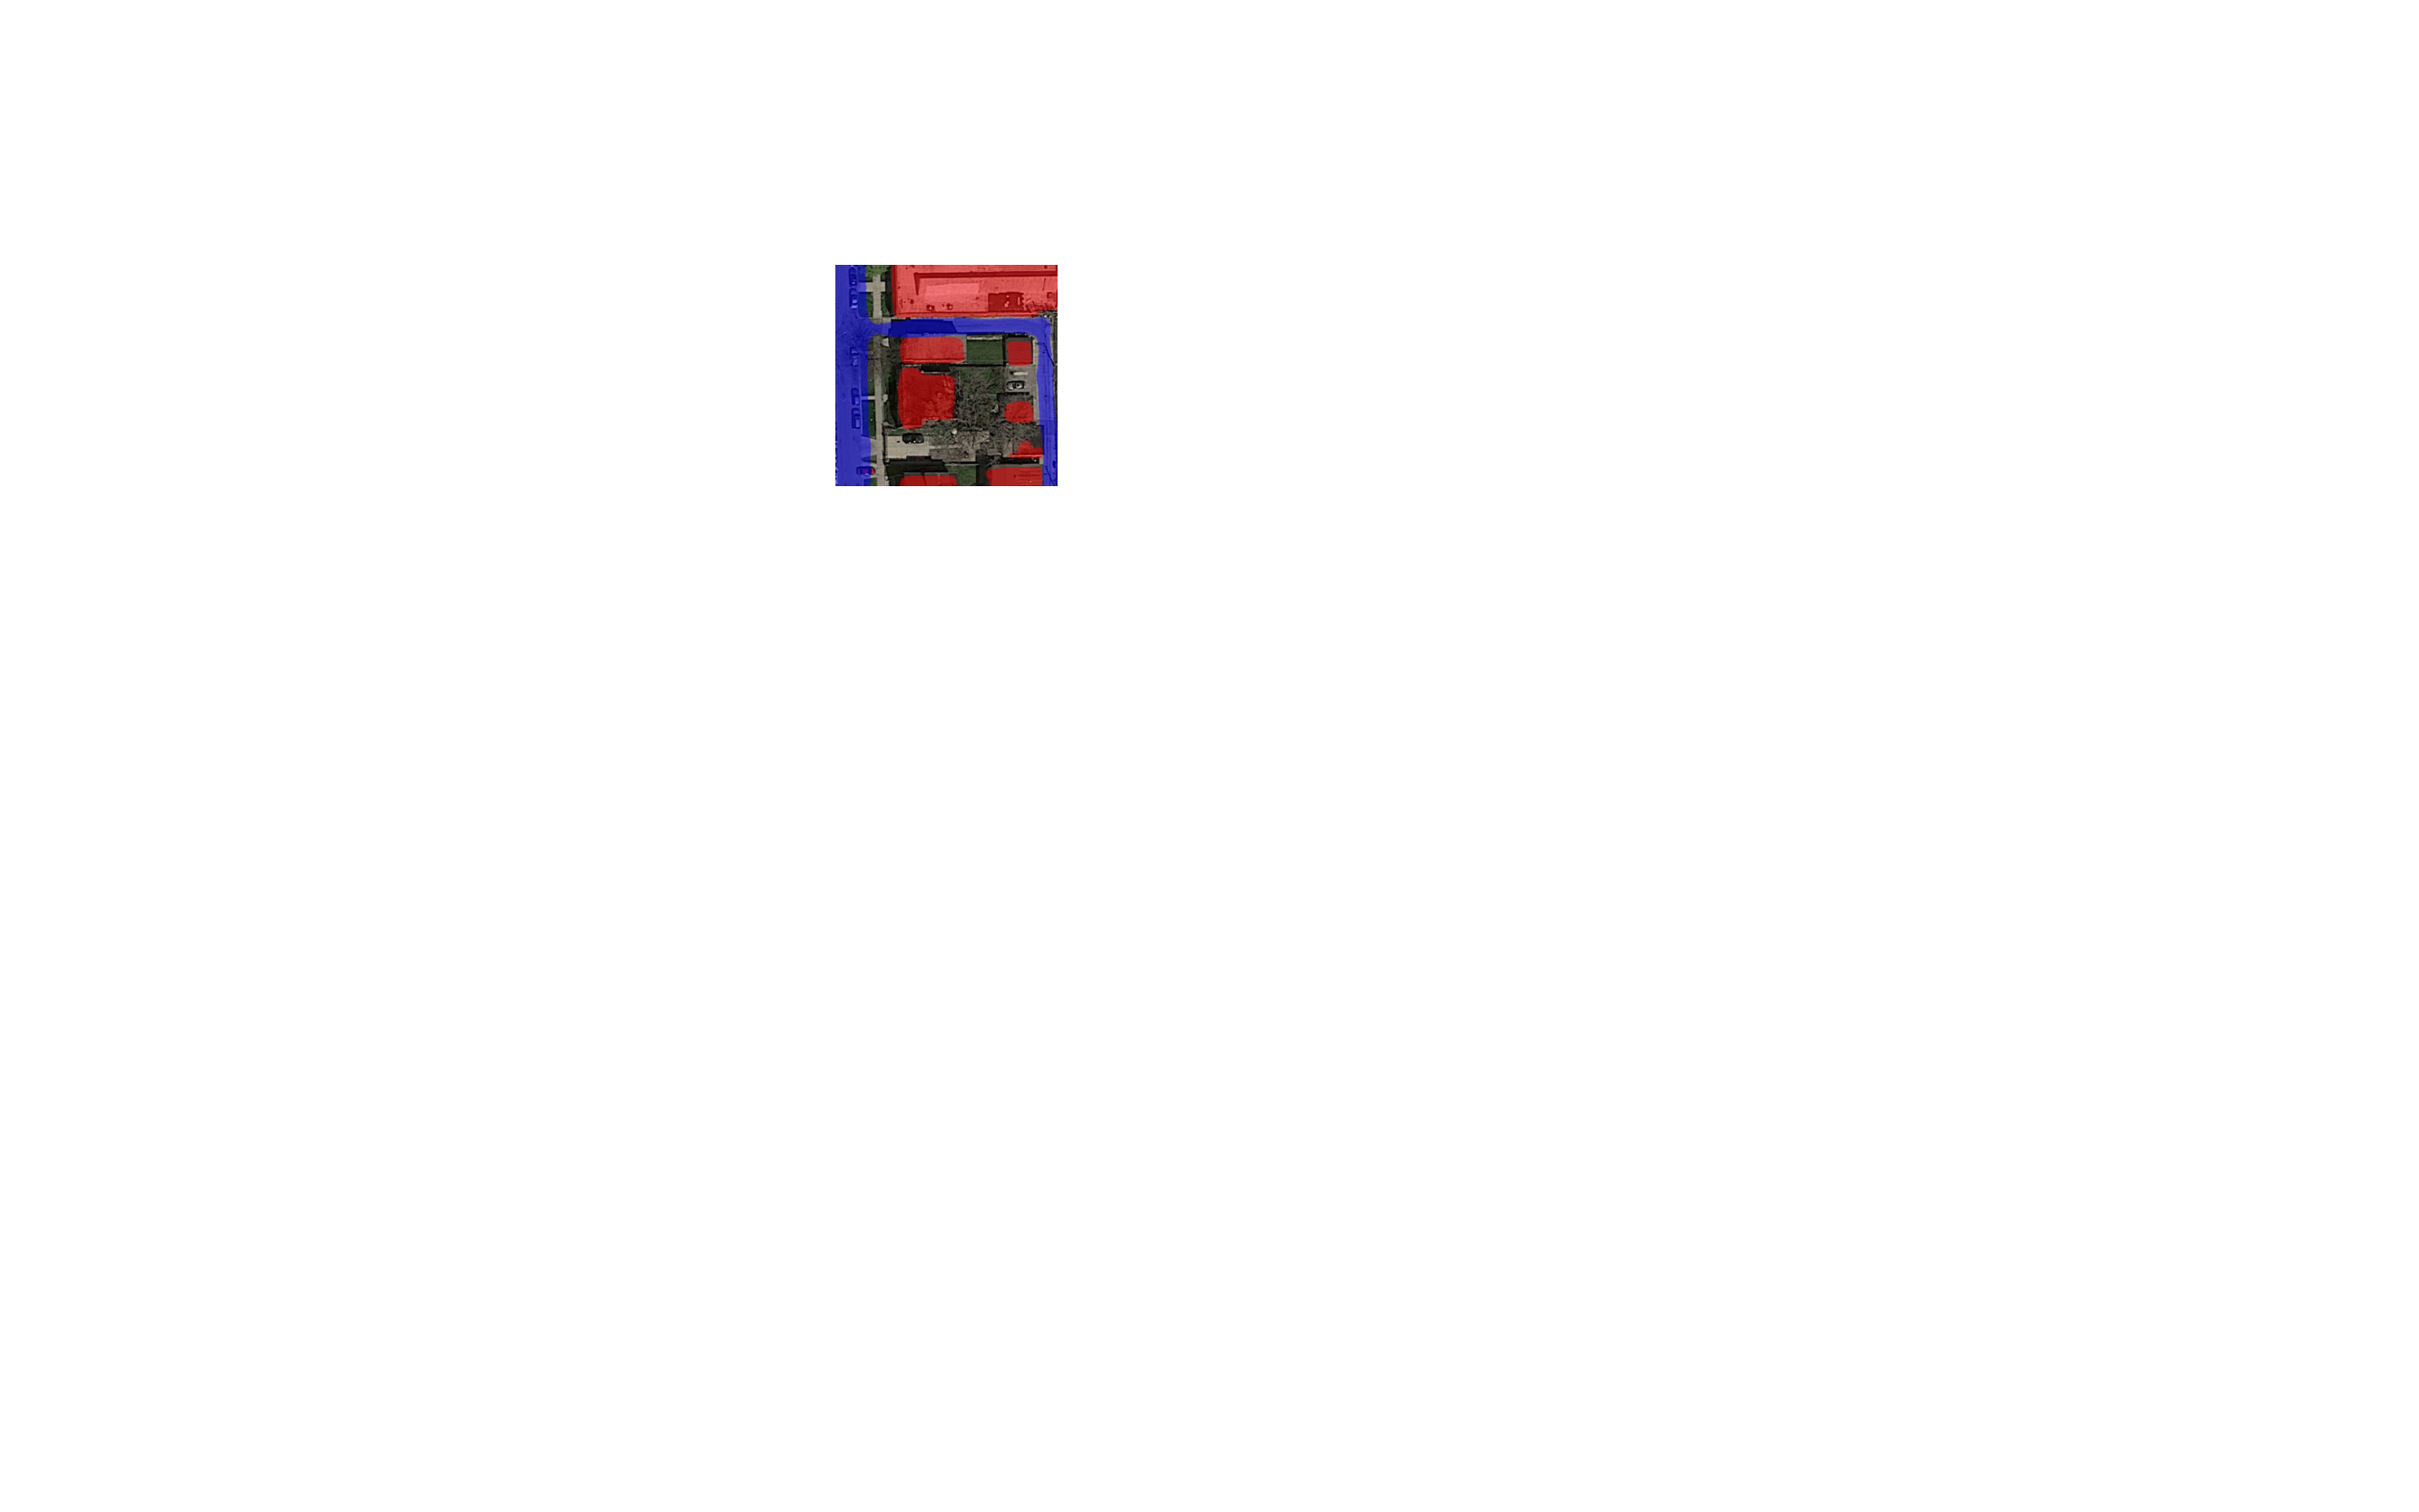
\includegraphics[width=\figfigfigfig\textwidth]{2-00-3.pdf}
	}
    \caption[Semantic segmentation in aerial images]{Semantic segmentation in aerial images. Image copyright owned by \cite{mspascal}. (a) and (c) are two aerial images. In the semantic segmentation result (b) and (d), the pixels covered by red color refer to buildings, while the pixels covered by blue color refer to roads.}
	\label{fig:mspascal}
\end{figure}



\paragraph{FCN for Aerial Images} In paper \cite{mspascal}, FCN is employed in semantic segmentation in aerial images. In this work, each pixel in the aerial image is classified as different labels, i.e. buildings, roads or background. The output of the model is a per-pixel labelled mask. An example is shown in figure \ref{fig:mspascal}. We can see that the model can well distinguish between buildings and roads. However, there are also some limitations in this method with regard to our problem: (1) There is no instance segmentation here, and the buildings cannot be detected unless we do further pixel connectivity detection; (2) There is no segmentation of geometrical shapes of the objects in this model. Therefore, this model cannot be fully used to solve our problems.

\subsection{Frameworks for Instance Segmentation}\label{dlistseg}
As mentioned in subsection \ref{imgseg}, instance segmentation stands at a higher level than semantic segmentation, which additionally combines object detection as a kind of ``preprocessing". In fact, current object detection methods using deep learning networks, such as Faster R-CNN \cite{fasterrcnn}, YOLO \cite{yolo}, SSD \cite{ssd}, are very mature already.

Driven by the effectiveness of these object detection networks mentioned above, many approaches to instance segmentation are based on segment proposals. Earlier methods such as DeepMask \cite{deepmask} and its following work such as paper \cite{pedroinsseg} and \cite{daiinsseg1} learn to propose segment candidates, which are then classified. Similarly, paper \cite{daiinsseg} comes up with a complex multiple-stage cascade that predicts segment proposals from bounding box proposals, also followed by classification. In these methods, ``segmentation precedes recognition, which is slow and less accurate," \cite{maskrcnn}.

Most recently, paper \cite{liinsseg} integrates the segment proposal system and object detection system for FCIS (Fully Convolutional Instance Segmentation). The core idea for this combined model is to ``predict a set of position-sensitive output channels fully convolutionally," \cite{maskrcnn}. These changes make the whole system faster and more efficient as these channels can predict object classes, boxes and masks simultaneously. But FCIS does not perform well on overlapping instances and creates odd edges, showing that ``it is challenged by the fundamental difficulties of segmenting instances," \cite{maskrcnn}.

Instead, here we would like to introduce a state-of-the-art framework for instance segmentation with classification, Mask R-CNN \cite{maskrcnn}. It is based on ``parallel prediction of masks and class labels, which is simpler and more flexible," \cite{maskrcnn}.

Mask R-CNN is a general framework for object instance segmentation and classification. It is the latest model in the R-CNN family, which includes R-CNN \cite{rcnn}, Fast R-CNN \cite{fastrcnn}, Faster R-CNN \cite{fasterrcnn} as well. Mask R-CNN can efficiently detect and classify objects in an image and generate a high-quality segmentation mask for each instance simultaneously. Figure \ref{fig:rcnnres} shows example results of Mask R-CNN. We can see from the figure that this model achieves excellent results. Figure \ref{fig:rcnnsimmod} shows the simplified model architecture of Mask R-CNN. Each part of the structure are illustrated in detail as follows.

\begin{figure}[!h]
	\centering
	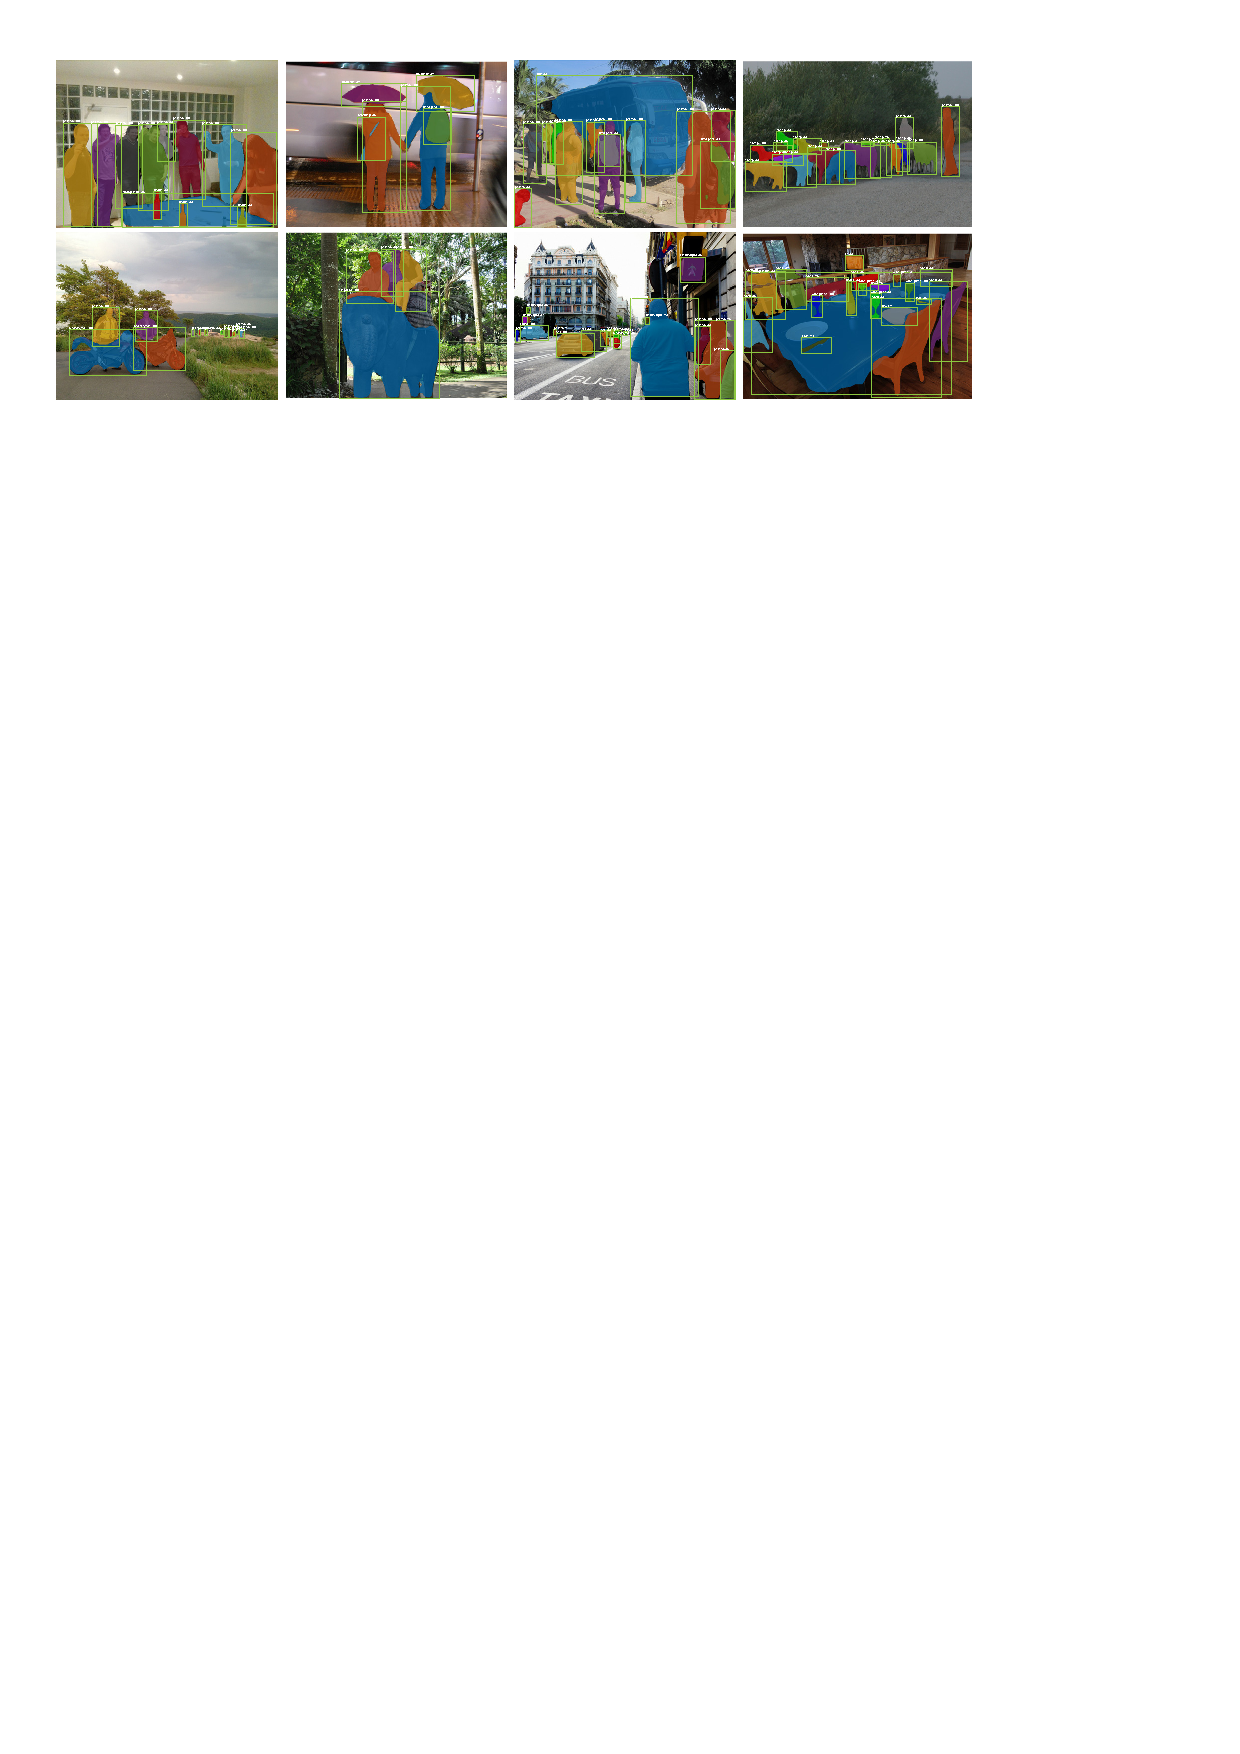
\includegraphics[width=\fig\textwidth]{2-02.pdf}
    \caption[Example results of Mask R-CNN]{Example results of Mask R-CNN.}
    \label{fig:rcnnres}
\end{figure}
\begin{figure}[!h]
	\centering
	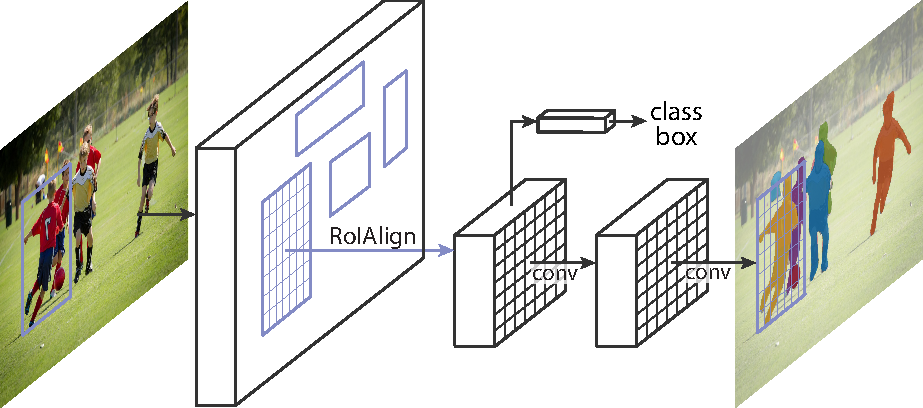
\includegraphics[width=\fig\textwidth]{2-03.pdf}
    \caption[Simplified model structure of Mask R-CNN]{Simplified model structure of Mask R-CNN. Feature Pyramid Network locates at the first layer in the figure.}
    \label{fig:rcnnsimmod}
\end{figure}

\paragraph{Feature Pyramid Network} The original image is first passed through the FPN (Feature Pyramid Network), which locates at the first layer in figure \ref{fig:rcnnsimmod}. FPN aims at finding multiple bounding boxes of the objects (known as RoIs, Regions of Interest) in the image. Actually, FPN can be regarded as an upgraded version of RPN (Region Proposal Network) used in Faster R-CNN \cite{fasterrcnn}. Compared with RPN, FPN introduces feature pyramid and solves the problem of multi-scale detection. Especially when the target object is relatively small, usually FPN would give better results than RPN, and thus improve the accuracy of detection. For more details about the model architecture of FPN, please refer to section \ref{modfpn}.

\paragraph{Classification Branch}
The classification branch exists from the earliest R-CNN \cite{rcnn} to the present Mask R-CNN \cite{maskrcnn}. It classifies each object in RoI found by FPN (or RPN in earlier models) as different classes and gives the probability distribution, using fully connected layers and softmax function. Note that this branch is not relevant to our problem, since currently we only interested in buildings rather than kinds of different objects in an aerial image.

\paragraph{Mask Branch}
Mask R-CNN extends Faster R-CNN by adding the mask branch for predicting an object mask on each RoI in parallel with the existing classification branch. This branch uses small FCN for the pixel-wise semantic segmentation, just like what we have already mentioned in subsection \ref{dlsemseg}. The mask branch should be relevant to our problem, but the mask it predicts is still in the pixel level instead of geometrical shape. \\

In short, Mask R-CNN can surpass prior instance segmentation results, but it cannot give any geometrical information of the objects in an image. Therefore, we consider that FPN is the only part in Mask R-CNN, which can be utilized to solve our problems. We hope that FPN can make correct detection of all buildings and localizing each using a bounding box. What we need to do next is to find appropriate methods for extracting geometrical shapes for each object detected.

\section{Frameworks Related to Geometrical Shapes}\label{frmgeo}
In this section, several frameworks which can find geometrical shapes are presented, including graph-based approach (see subsection \ref{graph}), polygonal partitioning approach (see subsection \ref{ppapp}), bounding box covering approach (see subsection \ref{bboxapp}) and PolygonRNN \cite{polygonrnn} (see subsection \ref{polygonrnn}) approach.

\subsection{Graph-based Approach}\label{graph}
The graph-based approach is proposed in the thesis work \cite{msnadine}, of which the pipeline is illustrated in figure \ref{fig:graphbased}. In this approach, buildings are regarded as polygons defined by corners and edges. The process of segmentation contains following steps: (1) Detect corners; (2) Compute the probability of two arbitrary different corners belonging to the same building; (3) Assemble over-complete set of potential corners and edges to a graph; (4) Segment graph into individual buildings.

\begin{figure}[!h]
	\centering
	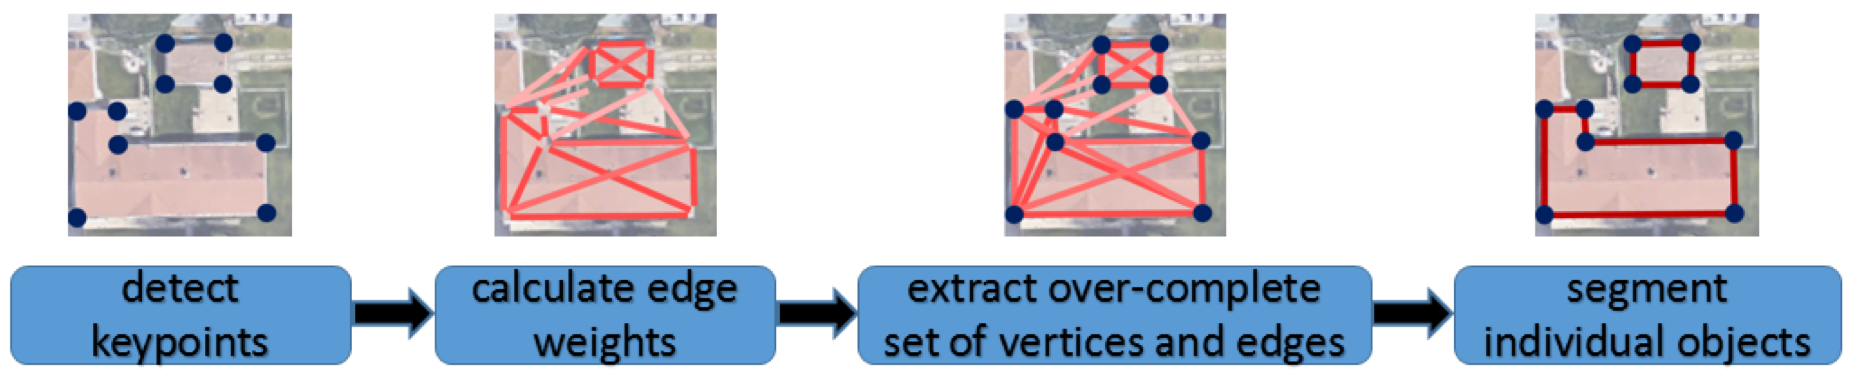
\includegraphics[width=\fig\textwidth]{2-07.png}
    \caption[Pipeline of graph-based approach for extracting polygons]{Pipeline of graph-based approach for extracting polygons. Image copyright owned by \cite{msnadine}.}
    \label{fig:graphbased}
\end{figure}

Actually, each stage of the graph-based approach has its own unsupervised solutions. For corner detection, we have Harris \cite{harris}, SIFT \cite{sift}, SURF \cite{surf} and so on. For the similarity of two image patches, we have histogram-based \cite{histbook} and BoW-based (Bag-of-Words-based) methods \cite{bow}. For graph segmentation, we have graph's minimum cut, and unsupervised learning approaches like spectral clustering.

However, each stage can also employ supervised learning methods, thus the parameters of each stage become learnable and trainable. Specifically, the thesis work \cite{msnadine} uses U-Net \cite{unet} as the corner detector, uses adapted siamese network (called ``triamese network" in the thesis work) described in \cite{siamese} to compute the probabilities for all potential corner pairs, and uses normalized cuts \cite{normcut} with its learning method \cite{normcutlearn} to segment individual objects. Figure \ref{fig:graphbased} shows two example results of the model, where the segmentation effect is just passable.

In addition, the thesis work does not provide more complicated situation, such as the number of building corners larger than four or the building not horizontally or vertically aligned. In theory, even if we find the vertices of an instance, it is also very difficult to determine their orders in order to form a polygon, which requires further processing.

\begin{figure}[!h]
	\centering
	\subbottom[\label{fig:graphbasedres1}]
		{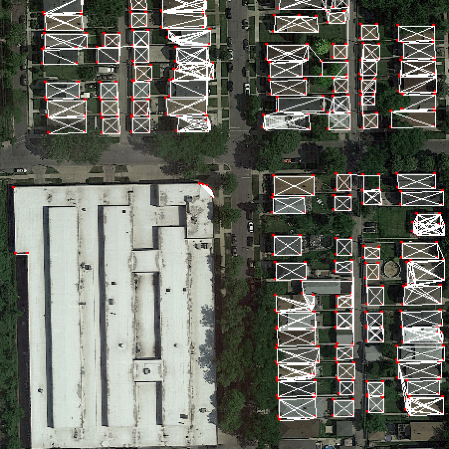
\includegraphics[width=\figfigfig\textwidth]{2-08-0.png}}
	\subbottom[\label{fig:graphbasedres2}]
		{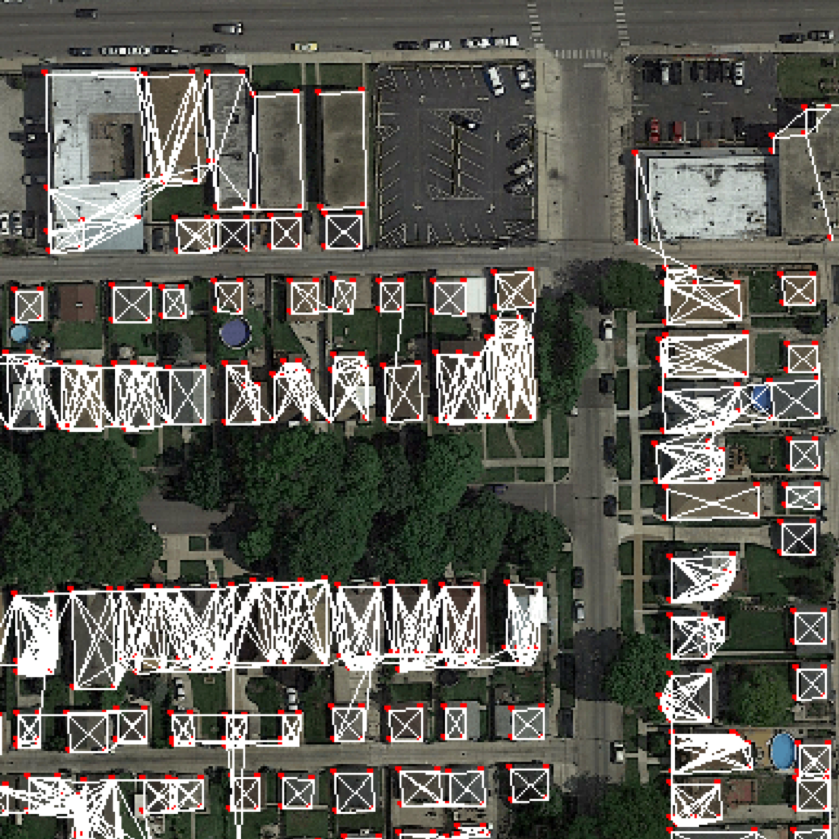
\includegraphics[width=\figfigfig\textwidth]{2-08-1.png}}
    \caption[Example results of graph-based approach]{Example results of graph-based approach. Image copyright owned by \cite{msnadine}.}
    \label{fig:graphbasedres}
\end{figure}

\subsection{Polygonal Partitioning Approach}\label{ppapp}
Many traditional image segmentation algorithms use superpixels. The paper \cite{kippi} points out that floating polygons can be an interesting alternative, especially for analyzing scenes with strong geometric signatures such as man-made environments (cityscapes or aerial images of city). The paper also shows that existing algorithms such as \cite{forsytheimgseg} and \cite{duanimgseg} produce homogeneously-sized polygons that fail to capture thin geometric structures and over-partition large uniform areas.

In order to tackle these problems, a kinetic approach, called KIPPI (KInetic Polygonal Partitioning of Images), is proposed in the paper, which brings more flexibility on polygon shape and size. The key idea consists in ``progressively extending pre-detected line-segments until they meet each other," \cite{kippi}. Figure \ref{fig:kippires} shows an input-output example of this algorithm.

\begin{figure}[!h]
	\centering
	\subbottom[original image\label{fig:kippires1}]
		{\includegraphics[width=\figfigfig\textwidth]{2-09-0.pdf}}
	\subbottom[KIPPI result\label{fig:kippires2}]
		{\includegraphics[width=\figfigfig\textwidth]{2-09-1.pdf}}
    \caption[Example result of KIPPI]{Example result of KIPPI. Image copyright owned by \cite{kippi}. The KIPPI algorithm decomposes the original image (a) into a partition of convex polygons shown in (b).}
    \label{fig:kippires}
\end{figure}

From the figure we can see that, different from general superpixel-based methods imposing homogeneously-sized regions, the polygons generated by KIPPI are ``more meaningful, capturing both large components and thin lineic structures that compose, for instance, urban scenes," \cite{kippi}. The paper's experiments demonstrate that output partitions both contain less polygons and better capture geometric structures than those delivered by existing methods.

\begin{figure}[!h]
	\centering
	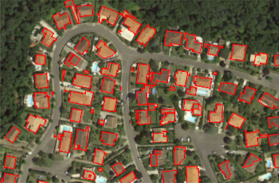
\includegraphics[width=\figfig\textwidth]{2-10.png}
    \caption[Segmenting buildings in an aerial image using KIPPI]{Segmenting buildings in an aerial image using KIPPI. Image copyright owned by \cite{kippi}.}
    \label{fig:kippiarlimg}
\end{figure}

Paper \cite{kippi} also show the applicative potential of the method when used as preprocessing in object contouring. To achieve polygonal object contouring from its partition, the paper associate each polygon with a binary activation variable indicating if it belongs to the objects of interest or not. The output polygonal contours correspond to the set of edges separating active polygons from inactive ones, which ensures that the contours are closed by construction. Figure \ref{fig:kippiarlimg} shows its application in segmenting buildings in an aerial image.

\subsection{Bounding Box Covering Approach}\label{bboxapp}
Additionally, the thesis work \cite{msnadine} proposes another approach, which we call bounding box covering approach. It utilizes the RPN in Faster R-CNN \cite{fasterrcnn} and additionally adds a branch for calculating the orientation degree. It predicts the rotated bounding box to best cover each building instance in an aerial image. Thus, the problem here becomes a parameters regression problem, which is to find out the center coordinates, width, height, and the rotation degrees of the bounding box. 

The model used here is the adapted RPN. As mentioned in subsection \ref{dlistseg}, the role of RPN in Faster R-CNN is to find RoIs, which are generally represented as bounding boxes or rectangles. This kind of representation can be very suitable for horizontally or vertically aligned buildings. But we know that buildings' orientations are not always regular, many of them are inclined in the image. Therefore, in this thesis project, RPN is adapted and another branch for rotating the bounding box is added. This can make the boundary of the bounding box closer to the building.

\begin{figure}[!h]
	\centering
	\subbottom[\label{fig:rotbbox1}]
		{\includegraphics[width=\figfig\textwidth]{2-11-0.pdf}}
	\subbottom[\label{fig:rotbbox2}]
		{\includegraphics[width=\figfig\textwidth]{2-11-1.pdf}}
    \caption[Example result of bounding box covering approach]{Example result of bounding box covering approach. Image copyright owned by \cite{msnadine}. The numbers shown in the figure indicate the probability that the rotated bounding box contains an object.}
    \label{fig:rotbbox}
\end{figure}

Figure \ref{fig:rotbbox} shows an example output. We can see from the figure that each building instance corresponds to a rotated bounding box, and is also limited tightly to the box. Results show that this method can detect buildings very well, but the geometrical shapes found are limited to rectangles and cannot be more precise for buildings that are not rectangular in shape.

\subsection{PolygonRNN}\label{polygonrnn}
PolygonRNN \cite{polygonrnn} aims at exploiting geometrical shape for single object instance within an image. The model is originally proposed for speeding up manually contouring the object since it can achieve semi-automatic annotation of object instances, but the model can also be used for geometrical segmentation for single instance as well.

Most current methods regard the instance segmentation problem as a pixel-wise classification problem, generally labeling each pixel as object or background (see figure \ref{fig:egpxlmsk} for example). Different from this traditional way, the paper treats the segmentation task as a polygon prediction problem. In particular, PolygonRNN takes the image of instance as input and sequentially produces vertices of the polygon outlining the object (see figure \ref{fig:egpoly} for example).

\begin{figure}[!h]
	\centering
	\subbottom[an example building\label{fig:egorgimg}]{
		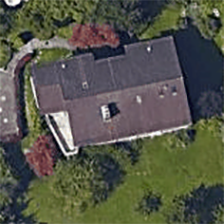
\includegraphics[width=\figfigfig\textwidth]{2-01-0.png}
	}
	\subbottom[per-pixel mask\label{fig:egpxlmsk}]{
		\frame{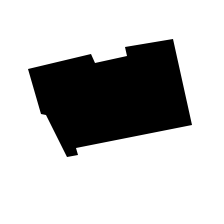
\includegraphics[width=\figfigfig\textwidth]{2-01-1.png}}
	}
	\subbottom[polygon representation\label{fig:egpoly}]{
		\frame{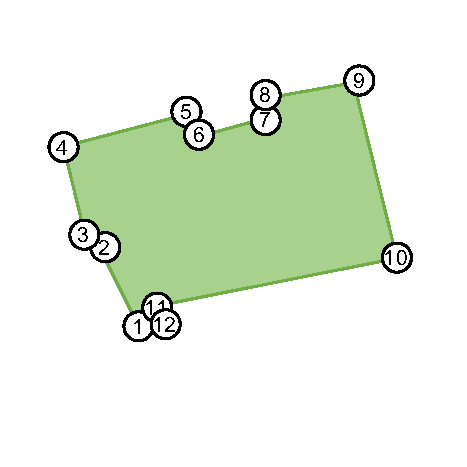
\includegraphics[width=\figfigfig\textwidth]{2-01-2.pdf}}
	}
    \caption[Comparison of pixel-wise mask and polygon]{Comparison of pixel-wise mask and polygon. (a) is the original image containing a building. (b) is the target mask of traditional pixel-wise instance segmentation, (c) is the desired prediction of polygon, of which the vertices are numbered.}
	\label{fig:egcmp}
\end{figure}

We know that predicting a polygon is equivalent to predicting each of its vertices. Thus, the paper regards polygon as a series of vertices, and uses RNN as the model to make coherent prediction. RNN is very powerful when data is related to time series as it can carry complex information about the history. In this case, the prediction of each vertex is dependent on the position of its two previous vertices. The paper also mentioned that another advantage over traditional methods is that RNN can capture the shape of the object even in ambiguous cases like shadows and saturation. In short, PolygonRNN can directly learn and predict the geometry of an object. For more details of the model architecture, please refer to section \ref{modpoly}.

\section{Motivation}\label{motivation}
Table \ref{tab:summod} makes a summary for all models introduced in this chapter.

\begin{table}[!h]
	\centering
	\caption[Summary of related work]{Summary of related work.}
	\label{tab:summod}
	\begin{tabularx}{\textwidth}{l|X|X|X|X}
	\hline
	\textbf{Model} & \textbf{Detection} & \textbf{Geometry} & \textbf{Classifica-tion} & \textbf{End-to-end} \\ \hline
	FCN \cite{fcn, mspascal} & Limited\footnotemark[1] & No & \textbf{Yes} & \textbf{Yes} \\
	Mask R-CNN \cite{maskrcnn} & \textbf{Yes} & No & \textbf{Yes} & \textbf{Yes} \\
	RPN \cite{fasterrcnn} or FPN \cite{fpn} & \textbf{Yes} & No & No & \textbf{Yes} \\ \hline
	Graph-based \cite{msnadine} & \textbf{Yes} & Limited\footnotemark[2] & No & No\footnotemark[3] \\
	KIPPI \cite{kippi} & Limited\footnotemark[4] & \textbf{Yes} & No & No\footnotemark[5]\\
	Adapted RPN \cite{msnadine} & \textbf{Yes} & Limited\footnotemark[6] & No & \textbf{Yes} \\
	PolygonRNN \cite{polygonrnn} & No & \textbf{Yes} & No & \textbf{Yes} \\ \hline
	\textbf{What We Want} & \textbf{Yes} & \textbf{Yes} & N/A\footnotemark[7] & \textbf{Yes} \\
	\hline
	\end{tabularx}
\end{table}
\footnotetext[1]{As mentioned in subsection \ref{imgseg}, object detection requires further processing of pixel connectivity detection.}
\footnotetext[2]{As mentioned in subsection \ref{graph}, the thesis work does not provide the result for more complicated geometry, and in theory, even if we find the vertices of an instance, it requires further processing to determine their orders to form a polygon.}
\footnotetext[3]{As mentioned in paper \cite{msnadine}, the whole model is a step-by-step process, each step is trained separately, so here we do not consider it is an end-to-end training.}
\footnotetext[4]{As mentioned in subsection \ref{ppapp}, the object outline is form by edges separating active and inactive polygons. However, differentiating multiple instances requires further detection of edge connectivity in the graph.}
\footnotetext[5]{Since detection and geometrical segmentation are both based on the polygonal partition result, here we do not regard it as an end-to-end training.}
\footnotetext[6]{As mentioned in section \ref{bboxapp}, the shape is only limited to rectangle.}
\footnotetext[7]{Segmentation for roads is currently not considered in our project, thus the cell here shows ``N/A", meaning not applicable.}

From the table we can conclude that none of these models meets our requirements. Thus, combination of two or even more models becomes necessary. After observation, we propose a possible approach, simply replacing the mask branch in Mask R-CNN with PolygonRNN and removing the classification branch, so that the adapted model can predict polygon rather than per-pixel mask for each RoI. This model takes advantages from both models, thus can be applied to our problem. In practice, we combine FPN and PolygonRNN and name it a new model \modelnameshort\ (\modelnamelong), of which the architecture is shown in detail in section \ref{modmer}.

